%%%%%%%%%%%%%%%%%%%%%%%%%%%%%%%%%%%%%%%%%%%%%%%%%%%%%%%%%%%%%%%%%%%%%%%%%%%%%%%%%%%%%%%%%%%%%%%%%%%%%%%%%%%%%%%%%%%%%%%%%%%%%%%%%%%%%%%%%%%%%%%%%%%%%%%%%%%%%%%%%%%
% Written By Michael Brodskiy
% Class: Embedded Design: Enabling Robotics
% Professor: S. Shazli
%%%%%%%%%%%%%%%%%%%%%%%%%%%%%%%%%%%%%%%%%%%%%%%%%%%%%%%%%%%%%%%%%%%%%%%%%%%%%%%%%%%%%%%%%%%%%%%%%%%%%%%%%%%%%%%%%%%%%%%%%%%%%%%%%%%%%%%%%%%%%%%%%%%%%%%%%%%%%%%%%%%

\include{Includes.tex}

\pagestyle{fancy}

\title{Multiplexers, Demultiplexers, Encoders, and Decoders}
\date{\today}
\author{Michael Brodskiy\\ \small Professor: S. Shazli}

\begin{document}

\maketitle

\thispagestyle{fancy}

\newpage

\begin{itemize}

  \item A multiplexer has:

    \begin{itemize}

      \item $N$ control inputs

      \item $2^N$ data inputs

      \item 1 output

    \end{itemize}

  \item A multiplexer routes (or connects) the selected data input to the output

    \begin{itemize}

      \item The value of the control inputs determines the data input that is selected

    \end{itemize}

    \begin{figure}[h!]
      \centering
      \tikzset{every picture/.style={line width=0.75pt}} %set default line width to 0.75pt        

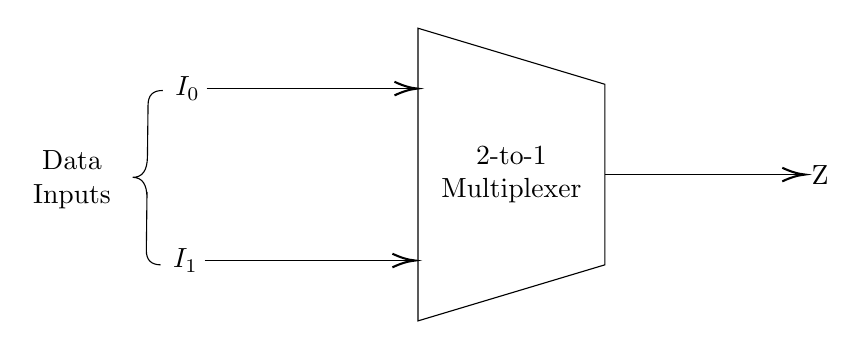
\begin{tikzpicture}[x=0.75pt,y=0.75pt,yscale=-1,xscale=1]
%uncomment if require: \path (0,642); %set diagram left start at 0, and has height of 642

%Shape: Trapezoid [id:dp36780303890607047] 
\draw   (223,53) -- (313,80) -- (313,167) -- (223,194) -- cycle ;
%Straight Lines [id:da433567050769597] 
\draw    (121.16,82.08) -- (220.58,82.08) ;
\draw [shift={(222.58,82.08)}, rotate = 180] [color={rgb, 255:red, 0; green, 0; blue, 0 }  ][line width=0.75]    (10.93,-3.29) .. controls (6.95,-1.4) and (3.31,-0.3) .. (0,0) .. controls (3.31,0.3) and (6.95,1.4) .. (10.93,3.29)   ;
%Straight Lines [id:da5507483232198851] 
\draw    (120.16,164.92) -- (219.58,164.92) ;
\draw [shift={(221.58,164.92)}, rotate = 180] [color={rgb, 255:red, 0; green, 0; blue, 0 }  ][line width=0.75]    (10.93,-3.29) .. controls (6.95,-1.4) and (3.31,-0.3) .. (0,0) .. controls (3.31,0.3) and (6.95,1.4) .. (10.93,3.29)   ;
%Shape: Brace [id:dp37108816823039836] 
\draw   (100,83) .. controls (95.33,82.95) and (92.97,85.25) .. (92.92,89.92) -- (92.62,114.92) .. controls (92.54,121.59) and (90.17,124.89) .. (85.5,124.83) .. controls (90.17,124.89) and (92.46,128.25) .. (92.38,134.92)(92.42,131.92) -- (92.09,159.92) .. controls (92.03,164.59) and (94.33,166.95) .. (99,167) ;
%Straight Lines [id:da2422167870643337] 
\draw    (313,123.5) -- (407.42,123.5) ;
\draw [shift={(409.42,123.5)}, rotate = 180] [color={rgb, 255:red, 0; green, 0; blue, 0 }  ][line width=0.75]    (10.93,-3.29) .. controls (6.95,-1.4) and (3.31,-0.3) .. (0,0) .. controls (3.31,0.3) and (6.95,1.4) .. (10.93,3.29)   ;

% Text Node
\draw (119.16,82.08) node [anchor=east] [inner sep=0.75pt]   [align=left] {$\displaystyle I_{0}$};
% Text Node
\draw (118.16,164.92) node [anchor=east] [inner sep=0.75pt]   [align=left] {$\displaystyle I_{1}$};
% Text Node
\draw (77.88,126) node [anchor=east] [inner sep=0.75pt]   [align=left] {\begin{minipage}[lt]{30.52pt}\setlength\topsep{0pt}
\begin{center}
Data\\Inputs
\end{center}

\end{minipage}};
% Text Node
\draw (411.42,123.5) node [anchor=west] [inner sep=0.75pt]   [align=left] {Z};
% Text Node
\draw (268,123.5) node   [align=left] {\begin{minipage}[lt]{52.04pt}\setlength\topsep{0pt}
\begin{center}
2-to-1\\Multiplexer
\end{center}

\end{minipage}};


\end{tikzpicture}

      \caption{A 2-to-1 Multiplexer}
      \label{fig:1}
    \end{figure}

    \begin{figure}[h!]
      \centering
      \include{Figures/4MUX}
      \caption{A 4-to-1 Multiplexer}
      \label{fig:2}
    \end{figure}

    \begin{figure}[h!]
      \centering
      \tikzset{every picture/.style={line width=0.75pt}} %set default line width to 0.75pt        

\begin{tikzpicture}[x=0.75pt,y=0.75pt,yscale=-1,xscale=1]
\path (0,642); %set diagram left start at 0, and has height of 642

%Shape: Trapezoid [id:dp36780303890607047] 
\draw   (223,53) -- (313,80) -- (313,338) -- (223,365) -- cycle ;
%Straight Lines [id:da433567050769597] 
\draw    (121.16,105.34) -- (220.58,105.34) ;
\draw [shift={(222.58,105.34)}, rotate = 180] [color={rgb, 255:red, 0; green, 0; blue, 0 }  ][line width=0.75]    (10.93,-3.29) .. controls (6.95,-1.4) and (3.31,-0.3) .. (0,0) .. controls (3.31,0.3) and (6.95,1.4) .. (10.93,3.29)   ;
%Straight Lines [id:da5507483232198851] 
\draw    (120.16,288.66) -- (219.58,288.66) ;
\draw [shift={(221.58,288.66)}, rotate = 180] [color={rgb, 255:red, 0; green, 0; blue, 0 }  ][line width=0.75]    (10.93,-3.29) .. controls (6.95,-1.4) and (3.31,-0.3) .. (0,0) .. controls (3.31,0.3) and (6.95,1.4) .. (10.93,3.29)   ;
%Shape: Brace [id:dp37108816823039836] 
\draw   (100,119.38) .. controls (95.33,119.36) and (92.99,121.68) .. (92.96,126.35) -- (92.55,202.28) .. controls (92.52,208.95) and (90.17,212.27) .. (85.5,212.24) .. controls (90.17,212.27) and (92.48,215.61) .. (92.44,222.28)(92.46,219.28) -- (92.03,298.22) .. controls (92,302.89) and (94.32,305.23) .. (98.99,305.26) ;
%Straight Lines [id:da2422167870643337] 
\draw    (313,209) -- (407.42,209) ;
\draw [shift={(409.42,209)}, rotate = 180] [color={rgb, 255:red, 0; green, 0; blue, 0 }  ][line width=0.75]    (10.93,-3.29) .. controls (6.95,-1.4) and (3.31,-0.3) .. (0,0) .. controls (3.31,0.3) and (6.95,1.4) .. (10.93,3.29)   ;
%Straight Lines [id:da3617010491941868] 
\draw    (121.16,166.95) -- (220.58,166.95) ;
\draw [shift={(222.58,166.95)}, rotate = 180] [color={rgb, 255:red, 0; green, 0; blue, 0 }  ][line width=0.75]    (10.93,-3.29) .. controls (6.95,-1.4) and (3.31,-0.3) .. (0,0) .. controls (3.31,0.3) and (6.95,1.4) .. (10.93,3.29)   ;
%Straight Lines [id:da5902913826647003] 
\draw    (121.16,228.91) -- (220.58,228.91) ;
\draw [shift={(222.58,228.91)}, rotate = 180] [color={rgb, 255:red, 0; green, 0; blue, 0 }  ][line width=0.75]    (10.93,-3.29) .. controls (6.95,-1.4) and (3.31,-0.3) .. (0,0) .. controls (3.31,0.3) and (6.95,1.4) .. (10.93,3.29)   ;
%Straight Lines [id:da10260405267377082] 
\draw    (120.16,136.34) -- (219.58,136.34) ;
\draw [shift={(221.58,136.34)}, rotate = 180] [color={rgb, 255:red, 0; green, 0; blue, 0 }  ][line width=0.75]    (10.93,-3.29) .. controls (6.95,-1.4) and (3.31,-0.3) .. (0,0) .. controls (3.31,0.3) and (6.95,1.4) .. (10.93,3.29)   ;
%Straight Lines [id:da030114751580914145] 
\draw    (119.16,319.66) -- (218.58,319.66) ;
\draw [shift={(220.58,319.66)}, rotate = 180] [color={rgb, 255:red, 0; green, 0; blue, 0 }  ][line width=0.75]    (10.93,-3.29) .. controls (6.95,-1.4) and (3.31,-0.3) .. (0,0) .. controls (3.31,0.3) and (6.95,1.4) .. (10.93,3.29)   ;
%Straight Lines [id:da21885134557568153] 
\draw    (120.16,197.95) -- (219.58,197.95) ;
\draw [shift={(221.58,197.95)}, rotate = 180] [color={rgb, 255:red, 0; green, 0; blue, 0 }  ][line width=0.75]    (10.93,-3.29) .. controls (6.95,-1.4) and (3.31,-0.3) .. (0,0) .. controls (3.31,0.3) and (6.95,1.4) .. (10.93,3.29)   ;
%Straight Lines [id:da1679293016464385] 
\draw    (120.16,259.91) -- (219.58,259.91) ;
\draw [shift={(221.58,259.91)}, rotate = 180] [color={rgb, 255:red, 0; green, 0; blue, 0 }  ][line width=0.75]    (10.93,-3.29) .. controls (6.95,-1.4) and (3.31,-0.3) .. (0,0) .. controls (3.31,0.3) and (6.95,1.4) .. (10.93,3.29)   ;

% Text Node
\draw (119.16,105.34) node [anchor=east] [inner sep=0.75pt]   [align=left] {$\displaystyle I_{0}$};
% Text Node
\draw (118.16,288.66) node [anchor=east] [inner sep=0.75pt]   [align=left] {$\displaystyle I_{6}$};
% Text Node
\draw (77.88,214.53) node [anchor=east] [inner sep=0.75pt]   [align=left] {\begin{minipage}[lt]{30.52pt}\setlength\topsep{0pt}
\begin{center}
Data\\Inputs
\end{center}

\end{minipage}};
% Text Node
\draw (411.42,209) node [anchor=west] [inner sep=0.75pt]   [align=left] {Z};
% Text Node
\draw (268,209) node   [align=left] {\begin{minipage}[lt]{52.04pt}\setlength\topsep{0pt}
\begin{center}
8-to-1\\Multiplexer
\end{center}

\end{minipage}};
% Text Node
\draw (119.16,166.95) node [anchor=east] [inner sep=0.75pt]   [align=left] {$\displaystyle I_{2}$};
% Text Node
\draw (119.16,228.91) node [anchor=east] [inner sep=0.75pt]   [align=left] {$\displaystyle I_{4}$};
% Text Node
\draw (118.16,136.34) node [anchor=east] [inner sep=0.75pt]   [align=left] {$\displaystyle I_{1}$};
% Text Node
\draw (117.16,319.66) node [anchor=east] [inner sep=0.75pt]   [align=left] {$\displaystyle I_{7}$};
% Text Node
\draw (118.16,197.95) node [anchor=east] [inner sep=0.75pt]   [align=left] {$\displaystyle I_{3}$};
% Text Node
\draw (118.16,259.91) node [anchor=east] [inner sep=0.75pt]   [align=left] {$\displaystyle I_{5}$};


\end{tikzpicture}

      \caption{A 8-to-1 Multiplexer}
      \label{fig:3}
    \end{figure}

  \item Example:

    \begin{itemize}

      \item Design a 4-to-1 multiplexer using 2-to-1 multiplexers only

      \item Essentially, ``stack'' three 2-to-1 multiplexers 

    \end{itemize}

\end{itemize}

\end{document}

